\documentclass{article}
\usepackage{amsmath}
\usepackage{tikz}
\usetikzlibrary{decorations.pathreplacing}

\begin{document}

\begin{center}
    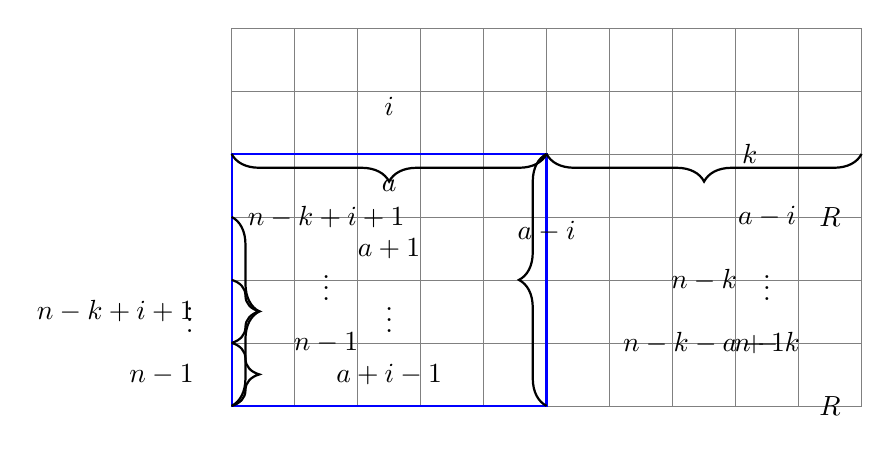
\begin{tikzpicture}[scale=0.8]
        % Draw the grid
        \draw[help lines] (0,0) grid (10,6);
        
        % Draw the rectangle R
        \draw[thick, blue] (0,0) rectangle (5,4);
        
        % Label the vertices of the rectangle r
        \node at (2.5,3.5) {$a$};
        \node at (2.5,2.5) {$a+1$};
        \node at (2.5,1.5) {$\vdots$};
        \node at (2.5,0.5) {$a+i-1$};
        
        % Label the vertices of the outer rectangle R
        \node at (9.5,3) {$R$};
        \node at (9.5,0) {$R$};
        
        % Draw the vertical steps
        \draw[decorate, decoration={brace, amplitude=10pt}, thick] (0,3) -- node[left=10pt] {$n-k+i+1$} (0,0);
        \draw[decorate, decoration={brace, amplitude=10pt}, thick] (0,2) -- node[left=10pt] {$\vdots$} (0,1);
        \draw[decorate, decoration={brace, amplitude=10pt}, thick] (0,1) -- node[left=10pt] {$n-1$} (0,0);
        
        % Draw the horizontal steps
        \draw[decorate, decoration={brace, mirror, amplitude=10pt}, thick] (5,4) -- node[above=10pt] {$a-i$} (5,0);
        \draw[decorate, decoration={brace, mirror, amplitude=10pt}, thick] (0,4) -- node[above=10pt] {$i$} (5,4);
        
        % Draw the label for the vertical steps
        \draw[decorate, decoration={brace, mirror, amplitude=10pt}, thick] (5,4) -- node[right=10pt] {$k$} (10,4);
        
        % Add labels for the horizontal steps
        \node at (7.5,2) {$n-k$};
        \node at (7.5,1) {$n-k-a+1$};
        
        % Add labels for the vertical steps
        \node at (1.5,3) {$n-k+i+1$};
        \node at (1.5,2) {$\vdots$};
        \node at (1.5,1) {$n-1$};
        
        % Add labels for the horizontal steps
        \node at (8.5,3) {$a-i$};
        \node at (8.5,2) {$\vdots$};
        \node at (8.5,1) {$n-k$};
        
    \end{tikzpicture}
\end{center}

The Pl\"ucker coordinate $\Delta_{I(r)}$ corresponding to a rectangle $r$ is given by the vertical steps in the path from the upper right corner to the lower left corner of the rectangle $R$ of size $k \times (n-k)$ that cuts out the rectangle $r$ positioned in the upper left corner of $R$.

\end{document}